
% :::::: III - Preliminaries ::::::::::::::::::
\section{Preliminaries}
\label{Preliminaries}
% no \IEEEPARstart
% This is section text. 

\subsection{Background}
% Establish the needed basics for the research
Handwriting recognition is the ability of a computer to retrieve and interpret handwriting input from sources such as paper documents, photographs, touch-screens and other devices. It is a classic machine learning problem  \cite{chen2014big}\cite{nair2015massively} with roots at least as far as the early 1900s, and the ideas have been applied to computer vision, speech, natural language processing, and other domains. For example, digit recognition has been employed regularly by the post office of all organizations, since the 1960s for the purposes of classifying street addresses using Optical Character Recognition.

Many algorithms have been proposed to solve this problem. Theoretically, every machine learning classification approach can be applied to this problem. From the basic linear classifier to advanced SVM approach, to recent neutral network approach, people keep improving the performance of handwritten digit classifier  \cite{peterson1989new}. One reason why people put in so much passion in this problem is because handwritten digit recognition can be regarded as the prototype of many complex recognition and classification problems. The success of classification of the handwritten digit dataset can be extended further to other advanced areas.

Recently, deep learning \cite{glorot2011domain}\cite{barrett2006researching} theory has been proposed to solve traditional machine learning problems, including image classification. One of the most important algorithms in this category is convolutional neutral network (CNN). It combines convolution operation with neutral network to extract local feature of 2D signal such as images and audio, and achieves quite promising result. In just a few years, such approach has been applied into many areas to solve different kind of problem.

%\begin {figure}[t]
%\centering
%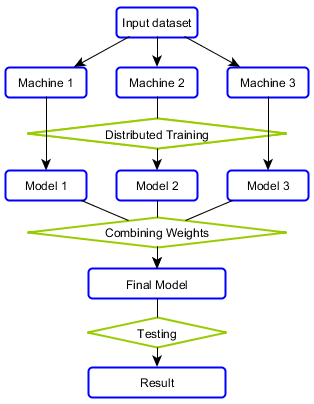
\includegraphics[width=0.9\columnwidth]{Figure1DistComArc.png} % REPLACED W/ BELOW
%%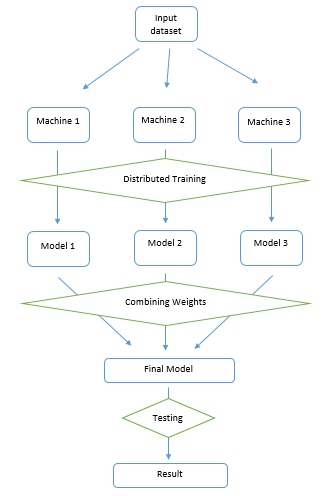
\includegraphics[width=7cm]{pic12.png}
%\caption{Distributed Computing Architecture}
%\label{Distributed Computing Architecture}
%\end {figure}

\begin {figure}[t]
\centering
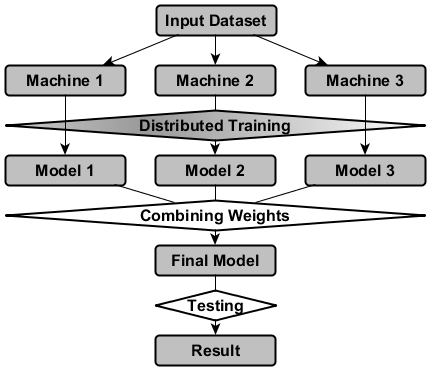
\includegraphics[width=0.90\columnwidth]{Paper_Fig1_DistCompArch.png}
%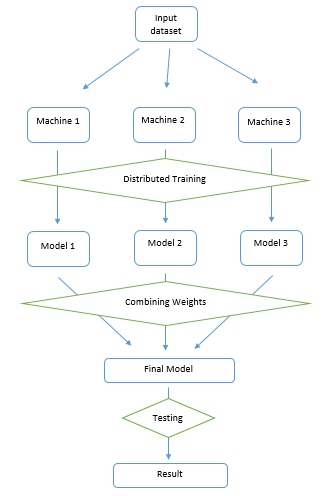
\includegraphics[width=7cm]{pic12.png}
%\vspace{-10pt}
\caption{Distributed Computing Architecture}
\label{Distributed Computing Architecture}
%\vspace{-10pt}
\end {figure}

There is no doubt about the performance of CNN, the problem is in actual application, it is intolerable to take one hour to recognize a ten-thousand article. On the condition of the high accuracy, time-cost is a significant concern before this algorithm goes out of labs. A balance between accuracy and cost is usual dilemma for classifier. To CNN it’s even more serious due to its incredible construction and calculation complexity.

Distributed computing system \cite{braun2001comparison}\cite{lawrence1997face} is common solution for big data. The idea is that we use multi-process on different CPUs with different machines \cite{morrison2005advancing}, which reduces the computations time in total \cite{lippmann1987introduction}. With proper implementation, we could separate the dataset and then combine the computed result together to make a reasonable model. Therefore, we decide to use this distributed computing to implement our CNN algorithm. 

Fig. \ref{Distributed Computing Architecture} shows our proposed solution. We begin by discretizing the input dataset and map each batch onto different machines. By CPU-based parallel computation \cite{li2013parameter}, we then train the CNN model with each batch of training data. After the training process, the parameters of the individual models are combined, creating one single (final) model. Finally, we test the final model to determine the accuracy and analyze the efficiency.


\subsection{Problem Definition}
\label{subsec:problem}
% Formalize the problem in terms of inputs, outputs, query/research-question, and objectives, e.g., reduce/min/max (accuracy, efficiency, distance, idle-time, etc)
\subsubsection{Inputs}
The input of our model is the handwritten digit dataset from the most widely used dataset website MNIST. It could be obtained
from \emph{http://yann.lecun.com/exdb/mnist/}.

The original black and white images from MNIST were normalized to fit in a 20x20 pixel box while preserving their aspect ratio. The resulting images contain grey levels as a result of the antialiasing technique used by the normalization algorithm. These images were centered in a 28x28 image by computing the center of mass of the pixels, and translating the image so as to position this point at the center of the 28x28 field.

\subsubsection{Outputs}
Given the input image, The output would be the classification result from the CNN model. To be more specific, the output is an integer from 1 to 9 inclusively, which indicates the digit in the image recognized by the algorithm.

In addition, in order to see the accuracy and efficiency, we also output the training time for certain number of iterations, and the accuracy after the entire training and testing process.
\subsubsection{Research Question}
With respect to improving classification problems implemented using a convolutional neural network (CNN), our research is centered around two important questions: (1) Can the classification accuracy be improved by introducing elastic distortion and noise to the original dataset? and (2) Does combining a distributed computing technique with the CNN model improve classification efficiency?

The handwritten digit recognition problem is the chosen case study upon which these questions are explored. 

\subsubsection{Objectives}
The objective is mainly about the accuracy and efficiency. Based on the elastic distortion, we try to improve the feature selection process, which makes the model more robust and improves the accuracy. As for the efficiency, the distribution would help us to reduce the computation time, so in future work more complicated model could be constructed if the computation complexity could be solved here.


% REMOVED THIS SECTION ---
% \subsection{Solution Architecture}
% \label{subsec:architecture}

%First, we implement the naive CNN algorithm with single process, as it is originally used. The CNN part is implemented by Python with Tensorflow library.  Tensorflow is an open source Python library developed by Google, which helps users to implement the deep learning algorithms in a more efficient way.
%Second, we add the distributed computing to the naive model. This process is also implemented by Python. The reason why we try to use the same programming language is to facilitate the calling and communication process between different languages which in turn will not require extra time. Using different programming languages may require extra computation time, which is a disadvantage. 
% MOVED BELOW

%To distribute the computation, we assign each machine with one batch of the input dataset. Then we run the training process on each machine with CPU-based computation. The connection between different machines is built by TCP/IP-based local area network. Fig. \ref{Solution Architecture for CNN with Distributed Computing} is a simple diagram that illustrates the solution architecture. 


% REMOVED THIS SECTION ---
% \subsection{Local Network System}
% \label{Local Network System}

%We build a TCP/IP-based local area network system to support the distribution computation process. Compared with ad-hoc, a server-client architecture is a more suitable choice because of MAP function and REDUCE function. A server takes charge of separation and distribution of incoming data which is a map function. Also it takes the responsibility to sum up sub-results from each single task. While clients work as typical mappers in MapReduce system handling one small part of the whole problem. 

%At start point, the server starts connections with clients and keep them online, followed by sending them data for the first round sequentially. Clients receive data and train model separately and return its final model parameters back to the server who collects and distribute a new section data to any unoccupied clients.

%TCP/IP (Transmission Control Protocol/Internet Protocol) is chosen as our communication protocol because of its error detection and correction. Data analysis is error sensitive while not much requirement for a high-speed transmission. Unlike UDP working without connection, TCP/IP also provides reliable connection and disconnection detection which is significant for a stable performance under an erratic or interrupted circumstance. 

%Steps to start this co-worker system are as followed. First, the server is needed to be started before any client begins so that it has time to make connection preparations finished and open a listening socket, waiting for connection requests. After that, clients are activated, sending connecting requests to the server according to the specific IP address and port number. 

%When an ask reaches the server, it tries to build a connection through three-time handshake and if succeed, the server creates a brand new socket specially sending and receiving data to and from this client. If the request is touched but no response or failure of connection, this request is going to be discard and that client has to send another connection request after a set time delay.

%As soon as a connection is built, the server grabs one part of the unsolved dataset and transmit to clients where input takes part in CNN model training processes. The server, on one side, keeps listening for potential connection request while on the other side, waits for result returning. Once a result comes back to the server, the feedback is expected to bring some contributions to final model i.e. added into summary CNN model for one step polish.

%The architecture of the {\em W} system is given in Figure~\ref{fig:architecture}.
% Describe briefly the main modules of the system and the employed data structures.
% We say briefly here as we will dedicate a separate section for each main module or part in the system.


% REMOVED THIS SECTION ---
% \subsection{Distributed Computing Model Justification}
% \label{Distributed Computing Model Justification}
% As mentioned in the introduction section, we need to prove that the combination of the distributed training results would be a reasonable model. We use this section to justify the model via mathematical deduction.

% The gradient descent method for updating parameters is used in the CNN model. The gradient descent direction found in each iteration is the direction that minimize the training error in each step. In the single computing method, the parameters are updated towards each gradient descent direction. From a mathematical perspective, it means we do an addition operation for every vector, which represents that direction.

% In our distributed computing method, we map each batch into different machines and do the training process simultaneously. With the same initial values, it can be seen as the decomposition of the vector from the initial value to the final value. The decomposed vectors are exactly the gradient descent vector calculated in each iteration. Since we use the same training dataset, and the batches are also the same for each iteration in the training process, it would result in the same weight as the single process model does. 

%% DELETED "Gradient Descent Method in CNN" figure
%\begin {figure}[t]
%\centering
%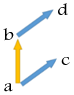
\includegraphics[width=1.5cm]{Fig3GradDes.png}
%\caption{Gradient Descent Method in CNN}
%\label{Gradient Descent Method in CNN}
%\end {figure}

% REMOVED THIS SECTION ---
% \subsection{Data Structures}
% \label{subsec:dataStructures}
% Provide detailed explanation about the employed or the introduced data structures here.
% For the input dataset, we reshaped the grey-value image matrix to a vector, and use one row to store it. Thus the whole dataset is represented as a matrix. As for the training process, we use the matrix computation through all the implementation part. The parameters in each layer are stored as a column in a big matrix, and the total matrix represents the weights for the entire neural network structure.

% Original text:
% For the input dataset, we use reshape the image grey value matrix to a vector, and use one row to store it. Thus the whole dataset is represented as a matrix. As for the training process, we use the matrix computation through all the implementation part. The parameters in each layer are stored as a column in a big matrix, and the total matrix represents the weights for the entire neural network structure.

% You can also make this subsection as a separate section or explain it while you are describing the other modules. This depends on how much contribution you did in the data structures.

% ======= END OF SECTION =======